\documentclass[10pt]{article}
\usepackage[top=50pt,bottom=50pt,left=48pt,right=46pt]{geometry}
\usepackage{color}
\usepackage[utf8]{inputenc}
\usepackage{float}
\usepackage[T1]{fontenc}
% \usepackage{indentfirst}
\usepackage{amsmath}
\usepackage{graphicx}
\usepackage{hyperref} 
% used for enumerate based on different symbols
% \begin{enumerate}[(a)] e.g.
\usepackage[shortlabels]{enumitem}

% beautifully indenting an environment
% \begin{addmargin}[1em]{2em}
% \end{addmargin}
% args: left margin, right margin
\usepackage{scrextend}

% for centered p columns in tabular environment
% \begin{tabular}{|P{2cm}|P{40mm}|P{4cm}|}
\usepackage{array}
\newcolumntype{P}[1]{>{\centering\arraybackslash}p{#1}}
\newcolumntype{M}[1]{>{\centering\arraybackslash}m{#1}}

% set paragraph indent to 0
% if you want to indent some paragraph, use \indentfirst command in front of them
\setlength{\parindent}{0pt}
\newcommand{\forceindent}{\leavevmode{\parindent=1em\indent}}


% for scaling a tabular table
\usepackage{graphicx}

\usepackage{listings}
% for code writing
% \begin{lstlisting}
% 	code here
% \end{lstlisting}
\lstset{
	breaklines=true,
	tabsize=2,
	basicstyle=\ttfamily,
}


% for comment block
\usepackage{verbatim}

% for debug purposes
% \usepackage{showframe}

% for setting section start value
\setcounter{section}{5}

% for code writing
% \begin{lstlisting} code here \end{lstlisting}
\usepackage{listings}
\lstset{
	% numbers=left,
	breaklines=true,
	tabsize=2,
	literate={\ \ }{{\ }}1,
	extendedchars=\true,
%	language=C,
	basicstyle=\footnotesize\ttfamily, 
%	stepnumber=1,
}



\newcommand{\indentitem}{\setlength\itemindent{25pt}}




% Title Page
\title{Implementation of Databases \\ ~~~ \\ Assignment 5 \\ ~~~ \\ }
\author{
	Participants:\\
	(sorted in last name order)\\
	Ulfet CETIN\\ 
	Shreya KAR\\
	Samuel ROY\\	
}
\date{}

\newlength{\mytab}
\setlength{\mytab}{1em}

\begin{document}

	\maketitle
	
	\clearpage
	
	\subsection*{Exercise 5.1 (Database Tuning)}
	
	\begin{enumerate}
		\item Draw the estimated execution plan for each query (i.e., an operator tree of algebra expressions
		and segment/index scans as it is provided by using the EXPLAIN statement in PostgreSQL).
		Estimate which query plan will perform better (Variant A or B) and argue why. You can
		use your favorite DBMS for this task, but we recommend PostgreSQL.
		
			
			\begin{itemize}
				\item Query 1A
				
				For each Computer Science course (a course from a department starting with ‘c’), get the
				course name and the average gpa of the students enrolled in the course.
				
						\begin{table}[H]
							\centering
							\scalebox{0.9}{
								\begin{tabular}{l l}
									SELECT 	& c.cname, AVG(s.gpa)\\
									FROM	& course c, enroll e, student s, dept d\\
									WHERE	& e.sid = s.sid AND c.did=d.did AND\\
											& d.dname LIKE 'c\%' AND\\
											& e.cid=c.cid\\
									GROUP BY& c.cid, c.cname;\\
								\end{tabular}
							}
						\end{table}
				
					\begin{figure}[h]
						\centering
						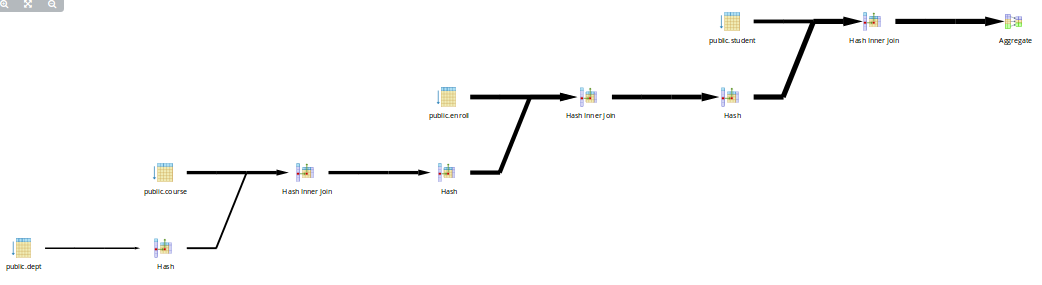
\includegraphics[scale=0.45]{query_plans/q1a.png}
						\caption{Query 1A Execution Plan}				
					\end{figure}
					
					\begin{center}
						\scalebox{0.75}{
				\begin{tabular}{l}
					\hspace{0\mytab} HashAggregate  (cost=23683.12..23752.56 rows=5555 width=113) (actual time=486.192..486.765 rows=2974 loops=1)\\
					\hspace{1\mytab} Group Key: c.cid, c.cname\\
					\hspace{1\mytab} ->  Hash Join  (cost=20233.34..23641.46 rows=5555 width=113) (actual time=330.505..431.874 rows=99059 loops=1)\\
					\hspace{2\mytab} Hash Cond: (s.sid = e.sid)\\
					\hspace{2\mytab} ->  Seq Scan on student s  (cost=0.00..2962.96 rows=103896 width=12) (actual time=0.009..10.256 rows=100000 loops=1)\\
					\hspace{2\mytab} ->  Hash  (cost=20163.90..20163.90 rows=5555 width=109) (actual time=330.379..330.379 rows=99059 loops=1)\\
					\hspace{3\mytab} Buckets: 32768 (originally 8192)  Batches: 4 (originally 1)  Memory Usage: 3841kB\\
					\hspace{3\mytab} ->  Hash Join  (cost=954.32..20163.90 rows=5555 width=109) (actual time=12.818..288.780 rows=99059 loops=1)\\
					\hspace{4\mytab} Hash Cond: (e.cid = c.cid)\\
					\hspace{4\mytab} ->  Seq Scan on enroll e  (cost=0.00..15404.25 rows=999925 width=8) (actual time=0.057..99.328 rows=999824 loops=1)\\
					\hspace{4\mytab} ->  Hash  (cost=952.19..952.19 rows=170 width=105) (actual time=12.730..12.730 rows=2974 loops=1)\\
					\hspace{5\mytab} Buckets: 4096 (originally 1024)  Batches: 1 (originally 1)  Memory Usage: 439kB\\
					\hspace{5\mytab} ->  Hash Join  (cost=12.26..952.19 rows=170 width=105) (actual time=0.059..11.460 rows=2974 loops=1)\\
					\hspace{6\mytab} Hash Cond: (c.did = d.did)\\
					\hspace{6\mytab} ->  Seq Scan on course c  (cost=0.00..823.62 rows=30562 width=109) (actual time=0.007..4.746 rows=30000 loops=1)\\
					\hspace{6\mytab} ->  Hash  (cost=12.25..12.25 rows=1 width=4) (actual time=0.022..0.022 rows=1 loops=1)\\
					\hspace{7\mytab} Buckets: 1024  Batches: 1  Memory Usage: 9kB\\
					\hspace{7\mytab} ->  Seq Scan on dept d  (cost=0.00..12.25 rows=1 width=4) (actual time=0.010..0.012 rows=1 loops=1)\\
					\hspace{8\mytab} Filter: (dname ~~ 'c\%'::text)\\
					\hspace{8\mytab} Rows Removed by Filter: 9\\
					\hspace{0\mytab} Planning time: 0.339 ms\\
					\hspace{0\mytab} Execution time: 487.036 ms\\
				\end{tabular}%
						}
					\end{center}
					
				\clearpage
					
				\item Query 1B
				
					\begin{table}[H]
						\centering
						\scalebox{0.9}{
							\begin{tabular}{l l}
								SELECT	& c2.cname, AVG(s.gpa)\\
								FROM	& enroll e, student s, course c2\\
								WHERE	& e.sid = s.sid AND\\
										&e.cid IN (SELECT cid FROM course c, dept d\\
								WHERE	& c.did=d.did AND d.dname LIKE 'c\%')\\
								GROUP BY& c2.cid, c2.cname;\\
							\end{tabular}
						}
					\end{table}
				
					\begin{figure}[h]
						\centering
						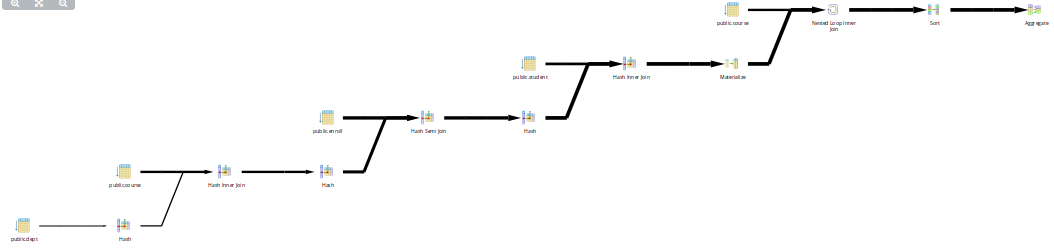
\includegraphics[scale=0.45]{query_plans/q1b.png}
						\caption{Query 1B Execution Plan}
					\end{figure}
					
					
					\begin{center}
						\scalebox{0.9}{
							\begin{tabular}{l}
								\hspace{0\mytab} GroupAggregate  (cost=70245800.20..72021223.18 rows=30562 width=113)\\
								\hspace{1\mytab} Group Key: c2.cid, c2.cname\\
								\hspace{1\mytab} ->  Sort  (cost=70245800.20..70689560.44 rows=177504096 width=113)\\
								\hspace{2\mytab} Sort Key: c2.cid, c2.cname\\
								\hspace{2\mytab} ->  Nested Loop  (cost=19120.58..2242170.57 rows=177504096 width=113)\\
								\hspace{3\mytab} ->  Seq Scan on course c2  (cost=0.00..823.62 rows=30562 width=105)\\
								\hspace{3\mytab} ->  Materialize  (cost=19120.58..22560.27 rows=5808 width=8)\\
								\hspace{4\mytab} ->  Hash Join  (cost=19120.58..22531.23 rows=5808 width=8)\\
								\hspace{5\mytab} Hash Cond: (s.sid = e.sid)\\
								\hspace{5\mytab} ->  Seq Scan on student s  (cost=0.00..2962.96 rows=103896 width=12)\\
								\hspace{5\mytab} ->  Hash  (cost=19047.98..19047.98 rows=5808 width=4)\\
								\hspace{6\mytab} ->  Hash Semi Join  (cost=954.32..19047.98 rows=5808 width=4)\\
								\hspace{7\mytab} Hash Cond: (e.cid = c.cid)\\
								\hspace{7\mytab} ->  Seq Scan on enroll e  (cost=0.00..15404.25 rows=999925 width=8)\\
								\hspace{7\mytab} ->  Hash  (cost=952.19..952.19 rows=170 width=4)\\
								\hspace{8\mytab} ->  Hash Join  (cost=12.26..952.19 rows=170 width=4)\\
								\hspace{9\mytab} Hash Cond: (c.did = d.did)\\
								\hspace{9\mytab} ->  Seq Scan on course c  (cost=0.00..823.62 rows=30562 width=8)\\
								\hspace{9\mytab} ->  Hash  (cost=12.25..12.25 rows=1 width=4)\\
								\hspace{10\mytab} ->  Seq Scan on dept d  (cost=0.00..12.25 rows=1 width=4)\\
								\hspace{11\mytab} Filter: (dname ~~ 'c\%'::text)\\
								\hspace{0\mytab} ERROR:  could not write block 4112449 of temporary file: No space left on device
						\end{tabular}%
					}
				\end{center}
				
				\clearpage
				
				\item Query 2A
				
				Get the names and departments of all courses with more than 40 students enrolled in them.
				
					\begin{table}[H]
						\centering
						\scalebox{0.9}{
							\begin{tabular}{l l}
							SELECT t.cname, t.dname\\
							FROM (SELECT c.cname, d.dname\\
							FROM enroll e, course c, dept d\\
							WHERE e.cid = c.cid AND d.did=c.did) AS t\\
							GROUP BY t.cname, t.dname\\
							HAVING COUNT(*) > 40;\\
							\end{tabular}
						}
					\end{table}
					
					\begin{figure}[h]
						\centering
						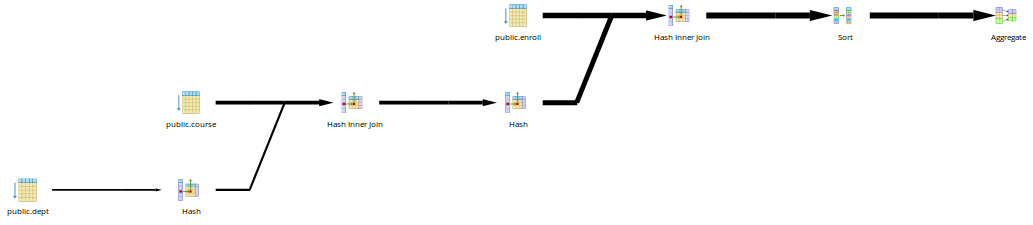
\includegraphics[scale=0.45]{query_plans/query2a.png}
						\caption{Query 2A Execution Plan}				
					\end{figure}
					
					\begin{center}
						\scalebox{0.8}{
							\begin{tabular}{l}
								\hspace{0\mytab} GroupAggregate  (cost=600229.97..622728.28 rows=999925 width=505) (actual time=7380.993..9506.403 rows=3299 loops=1)\\
								\hspace{1\mytab} Group Key: c.cname, d.dname\\
								\hspace{1\mytab} Filter: (count(*) > 40)\\
								\hspace{1\mytab} Rows Removed by Filter: 26701\\
								\hspace{1\mytab} ->  Sort  (cost=600229.97..602729.78 rows=999925 width=505) (actual time=7380.834..9174.248 rows=999824 loops=1)\\
								\hspace{2\mytab} Sort Key: c.cname, d.dname\\
								\hspace{2\mytab} Sort Method: external merge  Disk: 207184kB\\
								\hspace{2\mytab} ->  Hash Join  (cost=3639.92..42605.14 rows=999925 width=505) (actual time=25.343..837.752 rows=999824 loops=1)\\
								\hspace{3\mytab} Hash Cond: (e.cid = c.cid)\\
								\hspace{3\mytab} ->  Seq Scan on enroll e  (cost=0.00..15404.25 rows=999925 width=4) (actual time=0.048..143.019 rows=999824 loops=1)\\
								\hspace{3\mytab} ->  Hash  (cost=1257.90..1257.90 rows=30562 width=509) (actual time=25.134..25.134 rows=30000 loops=1)\\
								\hspace{4\mytab} Buckets: 8192  Batches: 8  Memory Usage: 986kB\\
								\hspace{4\mytab} ->  Hash Join  (cost=14.05..1257.90 rows=30562 width=509) (actual time=0.021..12.702 rows=30000 loops=1)\\
								\hspace{5\mytab} Hash Cond: (c.did = d.did)\\
								\hspace{5\mytab} ->  Seq Scan on course c  (cost=0.00..823.62 rows=30562 width=109) (actual time=0.005..3.325 rows=30000 loops=1)\\
								\hspace{5\mytab} ->  Hash  (cost=11.80..11.80 rows=180 width=408) (actual time=0.008..0.008 rows=10 loops=1)\\
								\hspace{6\mytab} Buckets: 1024  Batches: 1  Memory Usage: 10kB\\
								\hspace{6\mytab} ->  Seq Scan on dept d  (cost=0.00..11.80 rows=180 width=408) (actual time=0.002..0.004 rows=10 loops=1)\\
								\hspace{7\mytab} \\
								\hspace{0\mytab} Planning time: 0.175 ms\\
								\hspace{0\mytab} Execution time: 9540.965 ms\\
								
							\end{tabular}%
						}
					\end{center}
					
				\clearpage
				
				\item Query 2B
				
					\begin{table}[H]
						\centering
						\scalebox{0.9}{
							\begin{tabular}{l l}
								SELECT c.cname, d.dname\\
								FROM course c, dept d,\\
								(SELECT e.cid, COUNT(*) AS count\\
								FROM enroll e GROUP BY e.cid) AS t\\
								WHERE c.cid=t.cid AND c.did=d.did\\
								AND t.count > 40;\\
							\end{tabular}
						}
					\end{table}
					
					\begin{figure}[h]
						\centering
						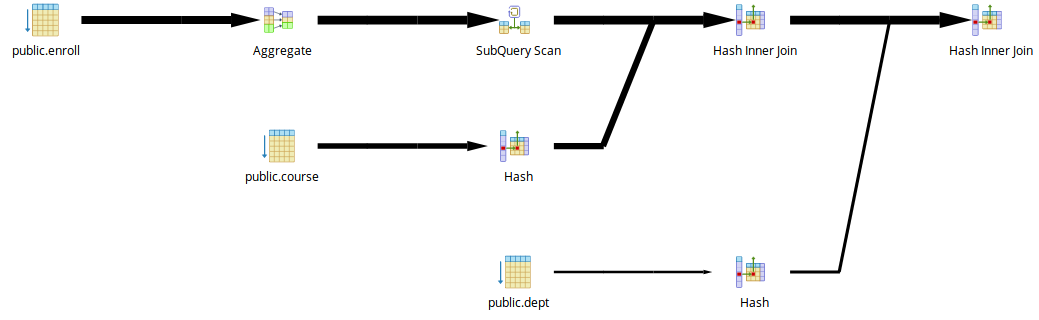
\includegraphics[scale=0.45]{query_plans/query2b.png}
						\caption{Query 2B Execution Plan}				
					\end{figure}
					
					\begin{center}
						\scalebox{0.8}{
							\begin{tabular}{l}
								\hspace{0\mytab} Hash Join  (cost=22131.57..24332.87 rows=29266 width=505) (actual time=464.619..475.965 rows=3299 loops=1)\\
								\hspace{1\mytab} Hash Cond: (c.did = d.did)\\
								\hspace{1\mytab} ->  Hash Join  (cost=22117.52..23916.41 rows=29266 width=105) (actual time=464.589..475.148 rows=3299 loops=1)\\
								\hspace{2\mytab} Hash Cond: (t.cid = c.cid)\\
								\hspace{2\mytab} ->  Subquery Scan on t  (cost=20403.88..21062.36 rows=29266 width=4) (actual time=446.831..453.419 rows=3299 loops=1)\\
								\hspace{3\mytab} ->  HashAggregate  (cost=20403.88..20769.70 rows=29266 width=4) (actual time=446.829..453.059 rows=3299 loops=1)\\
								\hspace{4\mytab} Group Key: e.cid\\
								\hspace{4\mytab} Filter: (count(*) > 40)\\
								\hspace{4\mytab} Rows Removed by Filter: 26701\\
								\hspace{4\mytab} ->  Seq Scan on enroll e  (cost=0.00..15404.25 rows=999925 width=4) (actual time=0.096..85.903 rows=999824 loops=1)\\
								\hspace{2\mytab} ->  Hash  (cost=823.62..823.62 rows=30562 width=109) (actual time=17.721..17.721 rows=30000 loops=1)\\
								\hspace{3\mytab} Buckets: 32768  Batches: 2  Memory Usage: 2370kB\\
								\hspace{3\mytab} ->  Seq Scan on course c  (cost=0.00..823.62 rows=30562 width=109) (actual time=0.004..6.519 rows=30000 loops=1)\\
								\hspace{1\mytab} ->  Hash  (cost=11.80..11.80 rows=180 width=408) (actual time=0.020..0.020 rows=10 loops=1)\\
								\hspace{2\mytab} Buckets: 1024  Batches: 1  Memory Usage: 10kB\\
								\hspace{2\mytab} ->  Seq Scan on dept d  (cost=0.00..11.80 rows=180 width=408) (actual time=0.009..0.012 rows=10 loops=1)\\
								\hspace{0\mytab} Planning time: 0.240 ms\\
								\hspace{0\mytab} Execution time: 476.373 ms\\
							\end{tabular}%
						}
					\end{center}
				
				\clearpage
				
				\item Query 3A
				
					\begin{table}[H]
						\centering
						\scalebox{0.9}{
							\begin{tabular}{l l}
								SELECT s.sname\\
								FROM \\
								student s\\
								WHERE s.sid IN (SELECT e.sid\\
								FROM enroll e GROUP BY e.sid\\
								HAVING COUNT(*)=(SELECT MAX(count)\\
								FROM(SELECT COUNT(*) as count\\
								FROM enroll e2\\
								GROUP BY e2.sid) AS foo));\\
							\end{tabular}
						}
					\end{table}
					
					\begin{figure}[h]
						\centering
						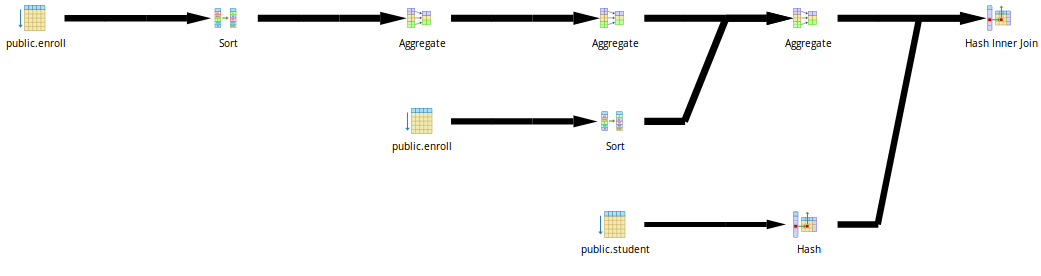
\includegraphics[scale=0.45]{query_plans/query3a.png}
						\caption{Query 3A Execution Plan}				
					\end{figure}
					
					\begin{center}
						\scalebox{0.8}{
							\begin{tabular}{l}
								\hspace{0\mytab} Hash Join  (cost=273062.40..286452.28 rows=51948 width=101) (actual time=2338.765..2763.940 rows=2 loops=1)\\
								\hspace{1\mytab} Hash Cond: (e.sid = s.sid)\\
								\hspace{1\mytab} ->  GroupAggregate  (cost=267075.74..275756.37 rows=94495 width=4) (actual time=2268.541..2711.911 rows=2 loops=1)\\
								\hspace{2\mytab} Group Key: e.sid\\
								\hspace{2\mytab} Filter: (count(*) = \$0)\\
								\hspace{2\mytab} Rows Removed by Filter: 99993\\
								\hspace{2\mytab} InitPlan 1 (returns \$0)\\
								\hspace{3\mytab} ->  Aggregate  (cost=138350.65..138350.66 rows=1 width=8) (actual time=1404.828..1404.828 rows=1 loops=1)\\
								\hspace{4\mytab} ->  GroupAggregate  (cost=128725.08..137169.47 rows=94495 width=4) (actual time=838.950..1396.571 rows=99995 loops=1)\\
								\hspace{5\mytab} Group Key: e2.sid\\
								\hspace{5\mytab} ->  Sort  (cost=128725.08..131224.89 rows=999925 width=4) (actual time=838.941..1256.485 rows=999824 loops=1)\\
								\hspace{6\mytab} Sort Key: e2.sid\\
								\hspace{6\mytab} Sort Method: external merge  Disk: 13632kB\\
								\hspace{6\mytab} ->  Seq Scan on enroll e2  (cost=0.00..15404.25 rows=999925 width=4) (actual time=0.045..127.181 rows=999824 loops=1)\\
								\hspace{2\mytab} ->  Sort  (cost=128725.08..131224.89 rows=999925 width=4) (actual time=833.346..1177.850 rows=999824 loops=1)\\
								\hspace{3\mytab} Sort Key: e.sid\\
								\hspace{3\mytab} Sort Method: external merge  Disk: 13632kB\\
								\hspace{3\mytab} ->  Seq Scan on enroll e  (cost=0.00..15404.25 rows=999925 width=4) (actual time=0.036..130.401 rows=999824 loops=1)\\
								\hspace{1\mytab} ->  Hash  (cost=2962.96..2962.96 rows=103896 width=105) (actual time=46.801..46.801 rows=100000 loops=1)\\
								\hspace{2\mytab} Buckets: 32768  Batches: 4  Memory Usage: 3700kB\\
								\hspace{2\mytab} ->  Seq Scan on student s  (cost=0.00..2962.96 rows=103896 width=105) (actual time=0.011..17.166 rows=100000 loops=1)\\
								\hspace{0\mytab} Planning time: 0.217 ms\\
								\hspace{0\mytab} Execution time: 2768.869 ms\\
							\end{tabular}%
						}
					\end{center}
				
				\clearpage
				
				\item Query 3B
				
					\begin{table}[H]
						\centering
						\scalebox{0.9}{
							\begin{tabular}{l l}
								SELECT s.sname FROM student s, enroll e\\
								WHERE s.sid=e.sid\\
								GROUP BY s.sid, s.sname\\
								HAVING COUNT(*) >= ALL\\
								(SELECT COUNT(*)\\
								FROM student s2, enroll e2\\
								WHERE s2.sid=e2.sid\\
								GROUP BY s2.sid);\\
							\end{tabular}
						}
					\end{table}
					
					\begin{figure}[h]
						\centering
						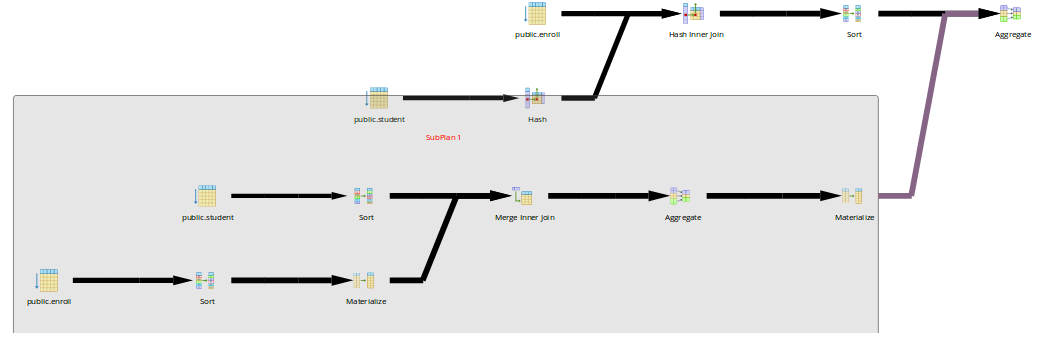
\includegraphics[scale=0.50]{query_plans/query3b.png}
						\caption{Query 3B Execution Plan}				
					\end{figure}
					
					\begin{center}
						\scalebox{0.8}{
							\begin{tabular}{l}
								\hspace{0\mytab} GroupAggregate  (cost=400878.81..1290586081.39 rows=103896 width=105) (actual time=4012.952..5099.537 rows=2 loops=1)\\
								\hspace{1\mytab} Group Key: s.sid, s.sname\\
								\hspace{1\mytab} Filter: (SubPlan 1)\\
								\hspace{1\mytab} Rows Removed by Filter: 99993\\
								\hspace{1\mytab} ->  Sort  (cost=260533.71..263033.52 rows=999925 width=105) (actual time=2182.442..2832.180 rows=999824 loops=1)\\
								\hspace{2\mytab} Sort Key: s.sid, s.sname\\
								\hspace{2\mytab} Sort Method: external merge  Disk: 115312kB\\
								\hspace{2\mytab} ->  Hash Join  (cost=5986.66..44676.88 rows=999925 width=105) (actual time=44.063..872.078 rows=999824 loops=1)\\
								\hspace{3\mytab} Hash Cond: (e.sid = s.sid)\\
								\hspace{3\mytab} ->  Seq Scan on enroll e  (cost=0.00..15404.25 rows=999925 width=4) (actual time=0.045..136.074 rows=999824 loops=1)\\
								\hspace{3\mytab} ->  Hash  (cost=2962.96..2962.96 rows=103896 width=105) (actual time=43.903..43.903 rows=100000 loops=1)\\
								\hspace{4\mytab} Buckets: 32768  Batches: 4  Memory Usage: 3715kB\\
								\hspace{4\mytab} ->  Seq Scan on student s  (cost=0.00..2962.96 rows=103896 width=105) (actual time=0.003..16.086 rows=100000 loops=1)\\
								\hspace{1\mytab} SubPlan 1\\
								\hspace{2\mytab} ->  Materialize  (cost=140345.11..164921.24 rows=103896 width=4) (actual time=0.009..0.019 rows=16 loops=99995)\\
								\hspace{3\mytab} ->  GroupAggregate  (cost=140345.11..164401.76 rows=103896 width=4) (actual time=906.078..1725.716 rows=99995 loops=1)\\
								\hspace{5\mytab} Group Key: s2.sid\\
								\hspace{5\mytab} ->  Merge Join  (cost=140345.11..158363.18 rows=999925 width=4) (actual time=906.064..1595.386 rows=999824 loops=1)\\
								\hspace{6\mytab} Merge Cond: (s2.sid = e2.sid)\\
								\hspace{6\mytab} ->  Sort  (cost=11619.98..11879.72 rows=103896 width=4) (actual time=65.760..81.434 rows=100000 loops=1)\\
								\hspace{7\mytab} Sort Key: s2.sid\\
								\hspace{7\mytab} Sort Method: external sort  Disk: 1368kB\\
								\hspace{7\mytab} ->  Seq Scan on student s2  (cost=0.00..2962.96 rows=103896 width=4) (actual time=0.009..13.892 rows=100000 loops=1)\\
								\hspace{6\mytab} ->  Materialize  (cost=128725.08..133724.70 rows=999925 width=4) (actual time=840.296..1341.554 rows=999824 loops=1)\\
								\hspace{7\mytab} ->  Sort  (cost=128725.08..131224.89 rows=999925 width=4) (actual time=840.292..1243.253 rows=999824 loops=1)\\
								\hspace{8\mytab} Sort Key: e2.sid\\
								\hspace{8\mytab} Sort Method: external merge  Disk: 13632kB\\
								\hspace{8\mytab} ->  Seq Scan on enroll e2  (cost=0.00..15404.25 rows=999925 width=4) (actual time=0.044..130.637 rows=999824 loops=1)\\
								\hspace{0\mytab} Planning time: 0.188 ms\\
								\hspace{0\mytab} Execution time: 5122.856 ms\\
							\end{tabular}
						}
					\end{center}
				
				\clearpage
				                                       
			\end{itemize}
			
			% query 1 comparison
			\begin{figure}[H]
				\begin{minipage}[]{0.45\linewidth}
					\begin{tabular}[t]{|c|c|c|}
						\hline
						Query Name: & Planning time & Execution time \\
						\hline
						Query 1A :  & 0.339 ms		& 487.036 ms\\ 
						Query 1B :  & no space		& no space \\
						\hline
					\end{tabular}
				\end{minipage}
				\hspace{0.1cm}
				\begin{minipage}[b]{0.55\linewidth}
					\begin{tabular}{p{0.95\linewidth}}
						\paragraph{Q1A}finishes with the values given on the right.
						\paragraph{Q1B}The reason why query 1b fails is because it runs out of memory in my setup (details given in %TODO)
						\paragraph{Conclusion} While Q1b did not even manage to return a result because it runs out of memory, Q1a returns the expected results. There is no comparison needed here.
					\end{tabular}
				\end{minipage}
			\end{figure}
			
			
			% query 2 comparison
			\begin{figure}[H]
				\begin{minipage}[]{0.45\linewidth}
					\begin{tabular}[t]{|c|c|c|}
						\hline
						Query Name: & Planning time & Execution time \\
						\hline
						Query 2A :  &  0.175 ms		& 9540.965 ms\\ 
						Query 2B :  &  0.240 ms		& 476.373 ms\\
						\hline
					\end{tabular}
				\end{minipage}
				\hspace{0.1cm}
				\begin{minipage}[b]{0.55\linewidth}
					\begin{tabular}{p{0.95\linewidth}}
						\paragraph{Q2A}has a multiple times(actually, near 20x) higher execution time due to having to sort on c.cname, d.dname using external merge. Using inner query is not a good idea on this type of retrieval.
						\paragraph{Q2B} has better overall score.
						\paragraph{Conclusion} Although q1b has considerably higher planning time, its execution time is multiple times(near 20x) better than the q1a. Therefore, the preferred query is \textbf{q1b}.
					\end{tabular}
				\end{minipage}
			\end{figure}
			
			% query 3 comparison
			\begin{figure}[H]
				\begin{minipage}[]{0.45\linewidth}
					\begin{tabular}[t]{|c|c|c|}
						\hline
						Query Name: & Planning time & Execution time \\
						\hline
						Query 3A :  &  0.217 ms		& 2768.869 ms\\ 
						Query 3B :  &  	0.188 ms	& 5122.856 ms\\
						\hline
					\end{tabular}
				\end{minipage}
				\hspace{0.1cm}
				\begin{minipage}[b]{0.55\linewidth}
					\begin{tabular}{p{0.95\linewidth}}
						\paragraph{Q3A} exploits the fact that being greater than the max of a list means being greater than all of the list, moreover, works on 94495 rows with width 4 when sorting/grouping, being the most costly step in this query.
						\paragraph{Q3B} works on 999925 rows with width 105 when sorting/grouping, being the most costly step in this query.
						\paragraph{Conclusion} q3a is nearly two times better than the query above, with the reasons and the numbers explained in the right and above.
					\end{tabular}
				\end{minipage}
			\end{figure}
			
			\bigskip
			
			\paragraph{The computer specification that the queries above are run at}:
				\begin{table}[H]
					\bigskip
					\scalebox{0.9}{
						\hspace*{5cm}
						\begin{tabular}{l l l}
							CPU 				&:& i5 5200U\\
							RAM 				&:& 8 GB DDR3\\
							HDD 				&:& 1 TB 5400 RPM SATA\\
							OS 					&:& Ubuntu 16.04 LTS\\
							PostgreSQL Version	&:& 9.5.14 on x86\_64-pc-linux-gnu\\
						\end{tabular}
					}
				\end{table}
			
			
			
			\clearpage
			
			\begin{comment}
				\begin{table}
				\footnotesize
				\begin{tabular}[t]{|c|c|c|}
				\hline
				Query Name: & Planning time & Execution time \\
				\hline
				Query 1A :  & 0.339 ms		& 487.036 ms\\ 
				Query 1B :  & no space		& no space \\
				\hline
				\end{tabular}
				\hfill
				\begin{tabular}[t]{|p{3.2cm}|c|}
				\hline
				bla&1\\ \hline
				blubb&2 \\ \hline
				bla&1\\ \hline
				blubb&2 \\ \hline   
				bla&1\\ \hline
				blubb&2 \\ \hline   
				\end{tabular}
				\hfill
				\begin{tabular}[t]{|p{3.2cm}|c|}
				\hline
				bla&1\\ \hline
				blubb&2 \\ \hline
				bla&1\\ \hline
				blubb&2 \\ \hline   
				bla&1\\ \hline
				blubb&2 \\ \hline   
				\end{tabular}
				\caption{99 most frequent hashtags in the data set.}
				\end{table}
			\end{comment}
			
			
			
			

			
			
			
			
			
			
		
		
		\item \underline{Performance Tuning} (6 pts)
		
		
		...Your task as a database administrator is to
		increase the performance for the given workload.\\
		Note: Include the updated SQL script of your submission.\\
		Make sure that the modified
		query really returns the same result as the original query (for all possible DB instances, not
		just for the provided sample databases).\\
		Please provide also Information about the result of
		genWorkload on your system and describe your system briefly (CPU, RAM, HDD or SSD).
		
		Consider the following informations for the Tuning Task:
		
		
		• The data is managed in a PostgreSQL server 10. The server has 8 GB of RAM and
		a CPU with 6 cores. There are also other applications running on this server, so you
		may not request all resources for the database server. The data is stored on classical
		hard disk (no SSD). You may change the configuration of your server (i.e., the file
		postgresql.conf); if you do so, explain your changes briefly in the PDF document, and
		include the modified postgresql.conf in the submitted ZIP file.
		
		• The database dump is available in L2P under Shared Documents. For testing, there are
		also smaller database dumps available. Note that you should first load the schema as
		the dump contains only data. You can use pgrestore (or the GUI pgadmin) to restore
		the database:
		pg\_restore --host localhost --port 5432 --username "postgres" --dbname "db"
		--no-password --section data "file.backup"
		
		• The workload is generated by the stored procedure genWorkload(N, Q). N is the
		number of statements which will be generated, and Q is the percentage of queries
		in the workload. In general, we assume that there are about 80% queries and 20%
		inserts, updates, and deletes. The genWorkload function will return the required in
		an exception message. The exception is raised to abort the transaction and to avoid a
		change in the database. Thus, you can repeatedly run the function without changing
		the database state. The goal is to minimize the time required for the query
		SELECT genWorkload(100,80). We recommend to start with the tiny database and
		smaller values for N , because without any optimizations or indexes, the workload might
		take hours or days.
		
		\clearpage
		
		\textbf{Optimizations}
		
		\begin{itemize}
			\item Changes in postgresql.conf
			
				\begin{enumerate}[1.]
					\item work\_mem parameter of PostgreSQL\\
					
					\textcolor{red}{Note:} even when I played with work\_mem parameters here, I could not manage to run q1b without running out of memory. Therefore, I am omitting q1b from the optimization, unfortunately.\\
					
					\begin{comment}
						pid  |    duration     |                                                                                                                       query                                                                                                                       | state  
						-------+-----------------+---------------------------------------------------------------------------------------------------------------------------------------------------------------------------------------------------------------------------------------------------+--------
						13919 | 00:06:12.504243 | EXPLAIN ANALYZE         SELECT c2.cname, AVG(s.gpa)     FROM enroll e, student s, course c2     WHERE e.sid = s.sid AND e.cid IN (SELECT cid FROM course c, dept d      WHERE c.did=d.did AND d.dname LIKE 'c%')        GROUP BY c2.cid, c2.cname | active
						14125 | 00:00:00        | SELECT                                                                                                                                                                                                                                           +| active
						|                 |   pid,                                                                                                                                                                                                                                           +| 
						|                 |   now() - pg_stat_activity.query_start AS duration,                                                                                                                                                                                              +| 
						|                 |   query,                                                                                                                                                                                                                                         +| 
						|                 |   state                                                                                                                                                                                                                                          +| 
						|                 | FROM pg_stat_activity;                                                                                                                                                                                                                            | 
						(2 rows)
					\end{comment}
					
					The default parameter is set to 4 MB.
					Increasing this size would greatly help. For this cause, I run a test suite which I build in Python. The test suite file, named dbTest.py can be found in the submission archive.\\
					
					* I run the test with different work\_mem values: [4,128,256,512,1024,2048] (values are in MBs)
					
					* Each query is run 5 times for each query, then the average is taken for that specific query.
					
					* After all queries are run five times for a specific work\_mem parameters and average is taken for each of the queries, averages of average of the queries is taken for that work\_mem value.\\
					
					Below is the result of the test suite:
					
					\begin{table}[H]
						\bigskip
						\scalebox{0.9}{
						\hspace*{2cm}
						\begin{tabular}{l|l|l|l|}
							\hline
							&Values for & Average List for Each MemSize & Avg. of the List \\
							\hline
							format:&how many MB set & [q1a, q2a, q2b, q3a, q3b averages] & average of averages \\
							\hline
							&4MB (default) 	& [375.2318, 8109.4804, 393.0298, 2247.0178, 6671.2208] & 3559.196 \\
							
							&128 MB 	& [476.1078, 10334.6318, 374.7442, 1056.6774, 2596.9826]&2967.828 \\
							&256 MB 	& [334.7756, 11805.4000, 390.1608, 1097.3964, 2663.1310] 	& 3258.172 \\
							&512 MB	& [341.2708, 5983.5754, 412.8676, 1064.0324, 2776.512] 	& 2115.651\\
							&1024 MB(first choice)	& [336.6438, 1523.5292, 390.6912, 1142.1504, 2730.2484]	&1224.652 \\
							&2048 MB & [340.7108, 1522.9682, 423.8814, 1074.005, 2834.3192] 	& 1239.176 \\ 
							\hline
						\end{tabular}
						}
					\end{table}
					
					We find here that 512 MB is not enough to really cut the costs, and 2048 MB is definitely not worth using compared to 1024 MB. But can we find a smaller value(512<x<1024) that allows us to get better results?
					
					\begin{table}[H]
						\bigskip
						\scalebox{0.9}{
							\hspace*{2cm}
							\begin{tabular}{l|l|l|l|}
								\hline
								&Values for & Average List for Each MemSize & Avg. of the List \\
								\hline
								format:&how many MB set & [q1a, q2a, q2b, q3a, q3b averages] & average of averages \\
								\hline
								&512MB	& [343.8215, 5349.1855, 387.3895, 1047.509, 2614.661] & 1948.5133 \\
								
								&600 MB 	& [334.79, 1461.262, 391.198, 1033.152, 2716.4045]& 1187.3613 \\
								&700 MB 	& [438.614, 1570.912, 402.4535, 1089.424, 2896.0145] 	& 1279.4836 \\
								&800 MB	& [354.703, 1531.719, 390.662, 1083.464, 2729.2005] 	& 1217.9497\\
								&900 MB(first choice)	& [361.186, 1463.753, 390.9565, 1049.192, 2700.947]	&1193.2069 \\
								&1000 MB & [344.709, 1517.286, 395.182, 1029.126, 2614.799] 	& 1180.2204 \\ 
								\hline
							\end{tabular}
						}
					\end{table}
					
					600 MB as work\_mem parameter is a good choice here.
					
					\bigskip
					
				\item shared\_buffer parameter of PostgreSQL\\
				
					As the machine specs given in the question body has 8 GB of RAM, I think the 2 GB of shared\_buffer value is a good choice for two things:
						
						\begin{itemize}[*]
							\item not all of the RAM of the system is given to the PostgreSQL.
							
							\item as given in the PostgreSQL documentation\footnote{PostGreSQL Version 9.5 Documentation: \url{https://www.postgresql.org/docs/9.5/runtime-config-resource.html}}:
							
							25\% of the main memory is a good choice for shared\_buffer parameter. Taken 8 GB main RAM into account, this makes 2 GB.
							
							\item we determined work\_mem as 600 MB, yet we are not given how many concurrent users will be active in the DB. Assuming there is no information on that(asked in L2P, waiting for answer), with 2 GB shared\_buffer value, at least 3 queries can be run in the server, which is a good value.
							
							Note that the query 1b, which causes the problem in the previous section, is runnable with this setup.
							
							
						\end{itemize}
						
					\bigskip
						
					\item rest of the parameters of PostgreSQL are left as they are.
					
					\clearpage
					
				\end{enumerate}
			
			\item Changes in the database itself
			
				\begin{enumerate}[1.]
					\item Materialized View structures in PostgreSQL are costly to update, as whenever the tables, which providing information to a materialized view, are updated, that materialized view has to be updated too. Moreover, we are not told whether we are allowed to modify the queries, therefore  we would assume that we cannot. If we cannot, there is no point in creating materialized views (as materialized views are just duplicate of the records, what SQL observes is that they are not another entities, "other tables".)
					\bigskip
					
					\item Indexes would be helpful.
					
					\begin{table}[H]
						\centering
						\begin{tabular}{|c | c | c | c | c | c | c|}
							\hline
							Query & student & dept & prof & course & major & enroll \\
							\hline
							Q1A & sid, gpa & did, dname & - & cid, cname, did & - & sid, cid\\
							Q1B & sid, gpa & did, dname & - & cid, cname, did & - & sid, cid\\
							\hline
							Q2A & - & did, dname & - & cid, cname & - & cid \\
							Q2B & - & did, dname & - & cid, cname & - & cid \\
							\hline
							Q3A & sid, sname & - & - & - & - & sid\\
							Q3B & sid, sname & - & - & - & - & sid\\
							\hline
						\end{tabular}
					\end{table}
					
					For query Q1A, the query optimizer makes use of:
					\begin{itemize}[*]
						\item CREATE INDEX course\_did ON course(did);
						\item CREATE INDEX enroll\_cid ON enroll(cid);
					\end{itemize}
					\bigskip
					
					For query Q1B, the query optimizer makes use of:
					\begin{itemize}[*]
						\item CREATE INDEX course\_cid\_cname ON course(cid, cname);
						\item CREATE INDEX course\_did ON course(did);
						\item CREATE INDEX enroll\_cid ON enroll(cid);
					\end{itemize}
					\bigskip
					
					For query Q3B, the query optimizer makes use of:
					\begin{itemize}[*]
						
						\item CREATE INDEX student\_sid ON student(sid);
						\item CREATE INDEX enroll\_sid ON enroll(sid);
					\end{itemize}
					\bigskip
					
					All the indexes used:
					\begin{itemize}[*]
						
						
						\item CREATE INDEX student\_sid ON student(sid);
						
						\item CREATE INDEX course\_did ON course(did);
						
						\item CREATE INDEX course\_cid\_cname ON course(cid, cname);
						
						\item CREATE INDEX enroll\_sid ON enroll(sid);
						
						\item CREATE INDEX enroll\_cid ON enroll(cid);
						
						\item CREATE INDEX enroll\_sid\_cid ON enroll(sid, cid);
					\end{itemize}
					
					
				\end{enumerate}
			
			
			
		\end{itemize}
		
		
		
		\clearpage
		\textbf{Final Conclusion}
		
		
		
		One can find all the changes we did to improve the DBMS performance:
		
		\begin{table}[H]
			\centering
			\begin{tabular}{|P{9.7cm} | P{4.4cm} | p{3.5cm} |}
				\hline
				&&Note that (80,20)\\
				Changes Made & genWorkload(80,20) Result &   here is just for trial\\
				& small\_dump & (look one page below \\
				&& for (100,80) )\\
				\hline
				\hline
				&&\\
				no changes & does not finish & \\
				&&\\
				\hline
				\hline
				&&\\
				\textbf{\underline{parameters changed:}} & & \\
				shared\_buffer = 2048 MB, & 1603086 ms & \\
				work\_mem = 600 MB & & \\
				&&\\
				\hline
				\hline
				&&\\
				\textbf{\underline{parameters changed:}} & & \\
				shared\_buffer = 2048 MB, & & \\
				work\_mem = 600 MB, & & \\
				&882692 ms&\\
				\textbf{\underline{optimization to DB:}} & & \\
				CREATE INDEX course\_cid\_cname ON course(cname, cid) &&\\
				&&\\
				\hline
				\hline
				&&\\
				\textbf{\underline{parameters changed:}} & & \\
				shared\_buffer = 2048 MB, & & \\
				work\_mem = 600 MB, & & \\
				&&\\
				\textbf{\underline{optimization to DB:}} & & \\
				
				CREATE INDEX student\_sid ON student(sid); &&\\
				&&\\
				
				CREATE INDEX course\_did ON course(did);&& from now on, this\\
				CREATE INDEX course\_cid\_cname ON course(cid, cname);& 636458 ms&will be called\\
				&& \textbf{\underline{final configuration}}\\
				
				CREATE INDEX enroll\_sid ON enroll(sid);&&\\
				CREATE INDEX enroll\_cid ON enroll(cid);&&\\
				CREATE INDEX enroll\_sid\_cid ON enroll(sid, cid);&&\\
				&&\\
				
				\textbf{\underline{changes in schema \& layout:}}&&\\
				each table has marked with its PRIMARY KEY,&& \\
				string fields shortened to save space and for less I/O&&\\
				(refer to the schema.sql file for more info) &&\\
				
				&&\\
				\hline
				
				
				
			\end{tabular}
			\vspace{1em}
			
			Defining foreign key constraints create problems when importing data, as data given to us are dumped without such constraints. pg\_restore retrieves tables in an order that does not match with the foreign key constraints.
			\bigskip
			
			Although pg\_restore can be imported, dumped back table by table, then can be imported partially, we believe that is not the point of this assignment. For this cause, we defined no foreign constraints in schema.sql file.
		\end{table}
		
		\begin{table}[H]
			\centering
			\begin{tabular}{|P{9.7cm} | P{6cm}|}
				\hline
				&\\
				dataset& genWorkload(100,80) Result\\
				&\\
				\hline
				
				&\\
				small\_dataset & 3291920 ms \\
				&\\
				\hline
				
				&\\
				medium\_dataset & did not finish\\
				&(run for more than 12 hours)\\
				&\\
				\hline
				
				&\\
				large\_dataset & \\
				&(like the medium dataset)\\
				\hline
				 
			\end{tabular}
			\vspace{3ex}
			
			Note that, the final configuration is used in this very table.
			
			Moreover, this time the function is run with the parameters given in the homework text ( e.g. genWorkload(100,80) )
		\end{table}
		
		\textbf{Summary}
		
		All the changes made:
		\begin{enumerate}
			\item PostgreSQL parameter optimization
			
			\item SQL Schemas primary key constraints
			
			(foreign key constraints omitted because of the restoring of the order of the tables does not match the foreign key constraints)
			
			\item SQL Schemas string fields shortened to reduce I/O times
			
			Initially all strings were of length 100, each table is analyzed to find the length of each string field (length of 50 at max). Then, to be on the safe side, each string fields is set to length of 55.
			
			\item SQL indexes are generated to aid the queries in the query optimizer.
		\end{enumerate}
		
		All the details on these changes can be found above and also in the schema.sql file.
		
	
		% comment on psql params
		\begin{comment}
		NOTICE:  1: Executing query 1
		NOTICE:  query 1: 1
		NOTICE:  2: Executing query 4
		NOTICE:  query 4: 39
		NOTICE:  3: Doing update 15
		NOTICE:  update 15: 1
		NOTICE:  4: Doing update 34
		NOTICE:  update 34: 24
		NOTICE:  5: Doing update 39
		NOTICE:  update 39: 45
		NOTICE:  6: Doing update 22
		NOTICE:  update 22: 0
		NOTICE:  7: Doing update 39
		NOTICE:  update 39: 26
		NOTICE:  8: Doing update 7
		NOTICE:  update 7: 1
		NOTICE:  9: Doing update 8
		NOTICE:  update 8: 0
		NOTICE:  10: Doing update 39
		NOTICE:  update 39: 35
		NOTICE:  11: Doing update 24
		NOTICE:  update 24: 229
		NOTICE:  12: Doing update 25
		NOTICE:  update 25: 191
		NOTICE:  13: Executing query 8
		NOTICE:  query 8: 12635
		NOTICE:  14: Executing query 2
		NOTICE:  query 2: 2
		NOTICE:  15: Doing update 21
		NOTICE:  update 21: 1
		NOTICE:  16: Doing update 18
		NOTICE:  update 18: 1108
		NOTICE:  17: Doing update 40
		NOTICE:  update 40: 29
		NOTICE:  18: Executing query 5
		NOTICE:  query 5: 117
		NOTICE:  19: Doing update 31
		NOTICE:  update 31: 2430
		NOTICE:  20: Doing update 31
		NOTICE:  update 31: 2183
		NOTICE:  21: Doing update 10
		NOTICE:  update 10: 35
		NOTICE:  22: Doing update 32
		NOTICE:  update 32: 2149
		NOTICE:  23: Doing update 38
		NOTICE:  update 38: 41
		NOTICE:  24: Doing update 29
		NOTICE:  update 29: 2198
		NOTICE:  25: Doing update 31
		NOTICE:  update 31: 2263
		NOTICE:  26: Executing query 11
		NOTICE:  query 11: 1299
		NOTICE:  27: Doing update 39
		NOTICE:  update 39: 50
		NOTICE:  28: Executing query 8
		NOTICE:  query 8: 322
		NOTICE:  29: Executing query 5
		NOTICE:  query 5: 129
		NOTICE:  30: Doing update 20
		NOTICE:  update 20: 45
		NOTICE:  31: Doing update 13
		NOTICE:  update 13: 134
		NOTICE:  32: Doing update 33
		NOTICE:  update 33: 55
		NOTICE:  33: Doing update 19
		NOTICE:  update 19: 903
		NOTICE:  34: Executing query 10
		NOTICE:  query 10: 1553136
		NOTICE:  35: Doing update 34
		NOTICE:  update 34: 64
		NOTICE:  36: Executing query 12
		NOTICE:  query 12: 422
		NOTICE:  37: Doing update 37
		NOTICE:  update 37: 60
		NOTICE:  38: Doing update 26
		NOTICE:  update 26: 272
		NOTICE:  39: Doing update 15
		NOTICE:  update 15: 0
		NOTICE:  40: Doing update 22
		NOTICE:  update 22: 0
		NOTICE:  41: Doing update 34
		NOTICE:  update 34: 58
		NOTICE:  42: Executing query 12
		NOTICE:  query 12: 367
		NOTICE:  43: Doing update 26
		NOTICE:  update 26: 200
		NOTICE:  44: Doing update 1
		NOTICE:  update 1: 0
		NOTICE:  45: Doing update 1
		NOTICE:  update 1: 1
		NOTICE:  46: Doing update 3
		NOTICE:  update 3: 0
		NOTICE:  47: Doing update 38
		NOTICE:  update 38: 55
		NOTICE:  48: Doing update 25
		NOTICE:  update 25: 203
		NOTICE:  49: Doing update 15
		NOTICE:  update 15: 0
		NOTICE:  50: Doing update 40
		NOTICE:  update 40: 59
		NOTICE:  51: Doing update 20
		NOTICE:  update 20: 55
		NOTICE:  52: Doing update 3
		NOTICE:  update 3: 0
		NOTICE:  53: Doing update 5
		NOTICE:  update 5: 0
		NOTICE:  54: Executing query 11
		NOTICE:  query 11: 1568
		NOTICE:  55: Doing update 37
		NOTICE:  update 37: 59
		NOTICE:  56: Doing update 15
		NOTICE:  update 15: 0
		NOTICE:  57: Doing update 32
		NOTICE:  update 32: 3774
		NOTICE:  58: Doing update 21
		NOTICE:  update 21: 0
		NOTICE:  59: Doing update 19
		NOTICE:  update 19: 1273
		NOTICE:  60: Doing update 24
		NOTICE:  update 24: 313
		NOTICE:  61: Doing update 26
		NOTICE:  update 26: 279
		NOTICE:  62: Doing update 33
		NOTICE:  update 33: 86
		NOTICE:  63: Executing query 4
		NOTICE:  query 4: 90
		NOTICE:  64: Doing update 3
		NOTICE:  update 3: 0
		NOTICE:  65: Doing update 35
		NOTICE:  update 35: 65
		NOTICE:  66: Doing update 8
		NOTICE:  update 8: 1
		NOTICE:  67: Executing query 11
		NOTICE:  query 11: 1663
		NOTICE:  68: Doing update 31
		NOTICE:  update 31: 3323
		NOTICE:  69: Doing update 28
		NOTICE:  update 28: 313
		NOTICE:  70: Doing update 1
		NOTICE:  update 1: 0
		NOTICE:  71: Doing update 27
		NOTICE:  update 27: 269
		NOTICE:  72: Doing update 14
		NOTICE:  update 14: 0
		NOTICE:  73: Executing query 11
		NOTICE:  query 11: 1779
		NOTICE:  74: Executing query 1
		NOTICE:  query 1: 0
		NOTICE:  75: Doing update 24
		NOTICE:  update 24: 262
		NOTICE:  76: Doing update 7
		NOTICE:  update 7: 0
		NOTICE:  77: Doing update 32
		NOTICE:  update 32: 3953
		NOTICE:  78: Doing update 34
		NOTICE:  update 34: 115
		NOTICE:  79: Doing update 37
		NOTICE:  update 37: 99
		NOTICE:  80: Doing update 12
		NOTICE:  update 12: 123
		NOTICE:  Time used: 1603086
		ERROR:  Workload completed after 1603086 ms, transaction aborted to avoid changes in DB
		\end{comment}
		
		
			% comment on clean run
		\begin{comment}
			
			NOTICE:  1: Executing query 1
			NOTICE:  query 1: 16
			NOTICE:  2: Executing query 4
			NOTICE:  query 4: 131
			NOTICE:  3: Doing update 15
			NOTICE:  update 15: 42
			NOTICE:  4: Doing update 34
			NOTICE:  update 34: 137
			NOTICE:  5: Doing update 39
			NOTICE:  update 39: 179
			NOTICE:  6: Doing update 22
			NOTICE:  update 22: 1
			NOTICE:  7: Doing update 39
			NOTICE:  update 39: 32
			NOTICE:  8: Doing update 7
			NOTICE:  update 7: 60
			NOTICE:  9: Doing update 8
			NOTICE:  update 8: 22
			NOTICE:  10: Doing update 39
			NOTICE:  update 39: 62
			NOTICE:  11: Doing update 24
			NOTICE:  update 24: 1560
			NOTICE:  12: Doing update 25
			NOTICE:  update 25: 687
			NOTICE:  13: Executing query 8
			NOTICE:  query 8: 32758
			NOTICE:  14: Executing query 2
			NOTICE:  query 2: 35
			NOTICE:  15: Doing update 21
			NOTICE:  update 21: 1
			NOTICE:  16: Doing update 18
			NOTICE:  update 18: 8594
			NOTICE:  17: Doing update 40
			NOTICE:  update 40: 32
			NOTICE:  18: Executing query 5
			NOTICE:  query 5: 11
			NOTICE:  19: Doing update 31
			NOTICE:  update 31: 2256
			NOTICE:  20: Doing update 31
			NOTICE:  update 31: 2278
			NOTICE:  21: Doing update 10
			NOTICE:  update 10: 51
			NOTICE:  22: Doing update 32
			NOTICE:  update 32: 2338
			NOTICE:  23: Doing update 38
			NOTICE:  update 38: 47
			NOTICE:  24: Doing update 29
			NOTICE:  update 29: 2398
			NOTICE:  25: Doing update 31
			NOTICE:  update 31: 3684
			NOTICE:  26: Executing query 11
			NOTICE:  query 11: 1433
			NOTICE:  27: Doing update 39
			NOTICE:  update 39: 51
			NOTICE:  28: Executing query 8
			NOTICE:  query 8: 328
			NOTICE:  29: Executing query 5
			NOTICE:  query 5: 11
			NOTICE:  30: Doing update 20
			NOTICE:  update 20: 41
			NOTICE:  31: Doing update 13
			NOTICE:  update 13: 1
			NOTICE:  32: Doing update 33
			NOTICE:  update 33: 51
			NOTICE:  33: Doing update 19
			NOTICE:  update 19: 1354
			NOTICE:  34: Executing query 10
			NOTICE:  query 10: 801721
			NOTICE:  35: Doing update 34
			NOTICE:  update 34: 56
			NOTICE:  36: Executing query 12
			NOTICE:  query 12: 342
			NOTICE:  37: Doing update 37
			NOTICE:  update 37: 56
			NOTICE:  38: Doing update 26
			NOTICE:  update 26: 475
			NOTICE:  39: Doing update 15
			NOTICE:  update 15: 0
			NOTICE:  40: Doing update 22
			NOTICE:  update 22: 0
			NOTICE:  41: Doing update 34
			NOTICE:  update 34: 55
			NOTICE:  42: Executing query 12
			NOTICE:  query 12: 339
			NOTICE:  43: Doing update 26
			NOTICE:  update 26: 470
			NOTICE:  44: Doing update 1
			NOTICE:  update 1: 1
			NOTICE:  45: Doing update 1
			NOTICE:  update 1: 0
			NOTICE:  46: Doing update 3
			NOTICE:  update 3: 0
			NOTICE:  47: Doing update 38
			NOTICE:  update 38: 57
			NOTICE:  48: Doing update 25
			NOTICE:  update 25: 432
			NOTICE:  49: Doing update 15
			NOTICE:  update 15: 0
			NOTICE:  50: Doing update 40
			NOTICE:  update 40: 58
			NOTICE:  51: Doing update 20
			NOTICE:  update 20: 44
			NOTICE:  52: Doing update 3
			NOTICE:  update 3: 0
			NOTICE:  53: Doing update 5
			NOTICE:  update 5: 1
			NOTICE:  54: Executing query 11
			NOTICE:  query 11: 1374
			NOTICE:  55: Doing update 37
			NOTICE:  update 37: 56
			NOTICE:  56: Doing update 15
			NOTICE:  update 15: 0
			NOTICE:  57: Doing update 32
			NOTICE:  update 32: 3719
			NOTICE:  58: Doing update 21
			NOTICE:  update 21: 0
			NOTICE:  59: Doing update 19
			NOTICE:  update 19: 1301
			NOTICE:  60: Doing update 24
			NOTICE:  update 24: 932
			NOTICE:  61: Doing update 26
			NOTICE:  update 26: 419
			NOTICE:  62: Doing update 33
			NOTICE:  update 33: 65
			NOTICE:  63: Executing query 4
			NOTICE:  query 4: 77
			NOTICE:  64: Doing update 3
			NOTICE:  update 3: 0
			NOTICE:  65: Doing update 35
			NOTICE:  update 35: 63
			NOTICE:  66: Doing update 8
			NOTICE:  update 8: 0
			NOTICE:  67: Executing query 11
			NOTICE:  query 11: 1377
			NOTICE:  68: Doing update 31
			NOTICE:  update 31: 2519
			NOTICE:  69: Doing update 28
			NOTICE:  update 28: 535
			NOTICE:  70: Doing update 1
			NOTICE:  update 1: 0
			NOTICE:  71: Doing update 27
			NOTICE:  update 27: 401
			NOTICE:  72: Doing update 14
			NOTICE:  update 14: 1
			NOTICE:  73: Executing query 11
			NOTICE:  query 11: 1375
			NOTICE:  74: Executing query 1
			NOTICE:  query 1: 0
			NOTICE:  75: Doing update 24
			NOTICE:  update 24: 928
			NOTICE:  76: Doing update 7
			NOTICE:  update 7: 0
			NOTICE:  77: Doing update 32
			NOTICE:  update 32: 2608
			NOTICE:  78: Doing update 34
			NOTICE:  update 34: 72
			NOTICE:  79: Doing update 37
			NOTICE:  update 37: 76
			NOTICE:  80: Doing update 12
			NOTICE:  update 12: 1
			NOTICE:  Time used: 882692
			ERROR:  Workload completed after 882692 ms, transaction aborted to avoid changes in DB
			\end{comment}
			
	
		
	\end{enumerate}
	
		\clearpage
		\subsection*{Exercise 5.2 (Query Optimization in MongoDB )}
		\begin{enumerate}
			\item Load the previous university data into MongoDB
			\begin{enumerate}
				\item A SQL script with CREATE TABLE flat (createFlatTbl.sql) is given on L2P, which
				stores the joined results of the four tables student, enroll, dept, course as Query1A from
				in Task 5.1.1 but without checking the department name. Execute the script; export the
				data in the table flat to a CSV file (e.g., flat.csv); create a new collection in MongoDB
				(e.g., also name it as flat) and load the data from flat.csv to this collection. (1 pts)
				
				Solution:
				\\1.Create db:
				\\>use my\_db
				\\2.Create Collection :
				\\>db.createCollection("flat")
				\\3.import data from csv file
				\\ mongoimport -d my\_db -c flat --type csv --file "/home/shreya/Documents/flat\_small.csv" --headerline
				
				

				\item  Write a MongoDB query Q5 on the new collection flat for the below requirement.
				Provide the query execution time. (Note in the new collection flat it already contains
				the joined results from original four tables.) (3 pts)
				(Q5) For each Computer Science course (a course from a department starting with c),
				get the course id and the average gpa of the students enrolled in the course.
				
				Solution:
				\\Query to execute aggregate function:
				
				$
				\\db.flat.aggregate([
				\\\{\$match: 
				    \\\{"dname":
				    /\string^c/\}\},\{\$group : \\\{\_id:"\$courseid",avg\_gpa:
				    \\\{\$avg : "\$gpa"\}\}\},
				    \\\{\$project : \{\_id:1, avg\_gpa:1, \}
				\\\}])
				$
				\\
				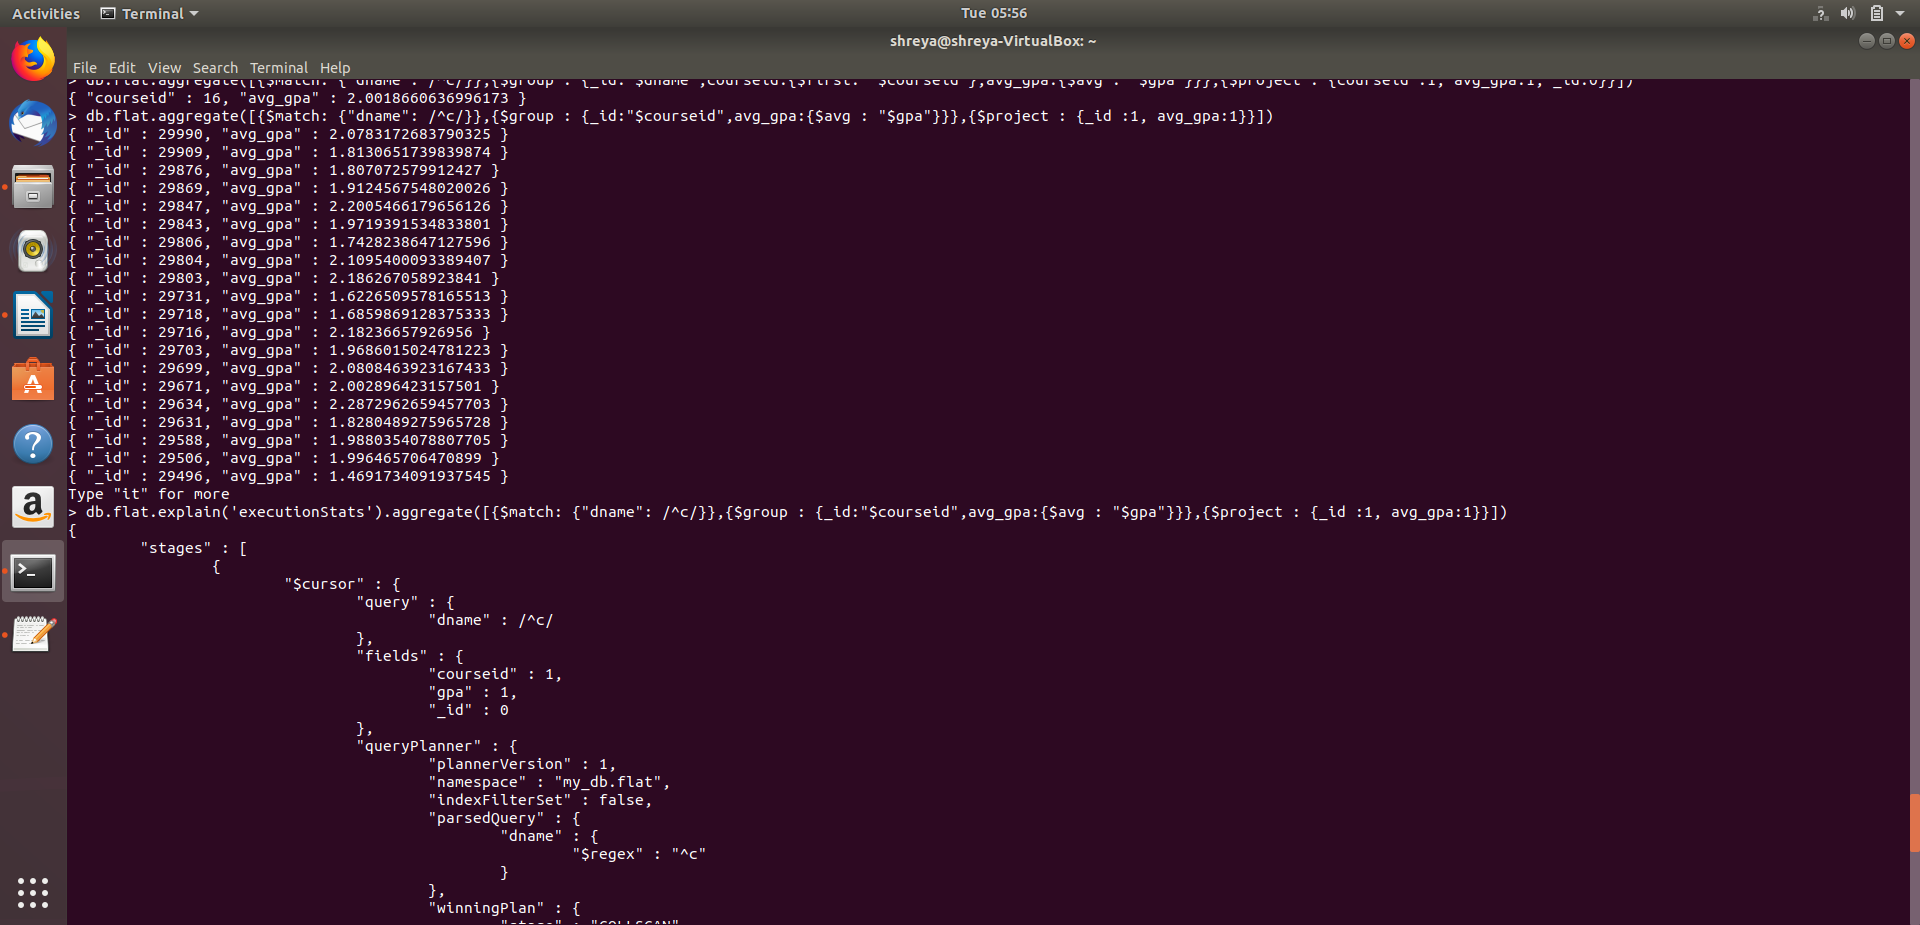
\includegraphics[scale=0.30]{mongo_1.png}
				
				execution time was 1634 ms 
				calculated by following query:
				$
				\\db.flat.explain('executionStats').aggregate([
				\\\{\$match: 
				    \\\{"dname":
				    /\string^c/\}\},\{\$group : \\\{\_id:"\$courseid",avg\_gpa:
				    \\\{\$avg : "\$gpa"\}\}\},
				    \\\{\$project : \{\_id:1, avg\_gpa:1, \}
				\\\}])
				$
				\\
				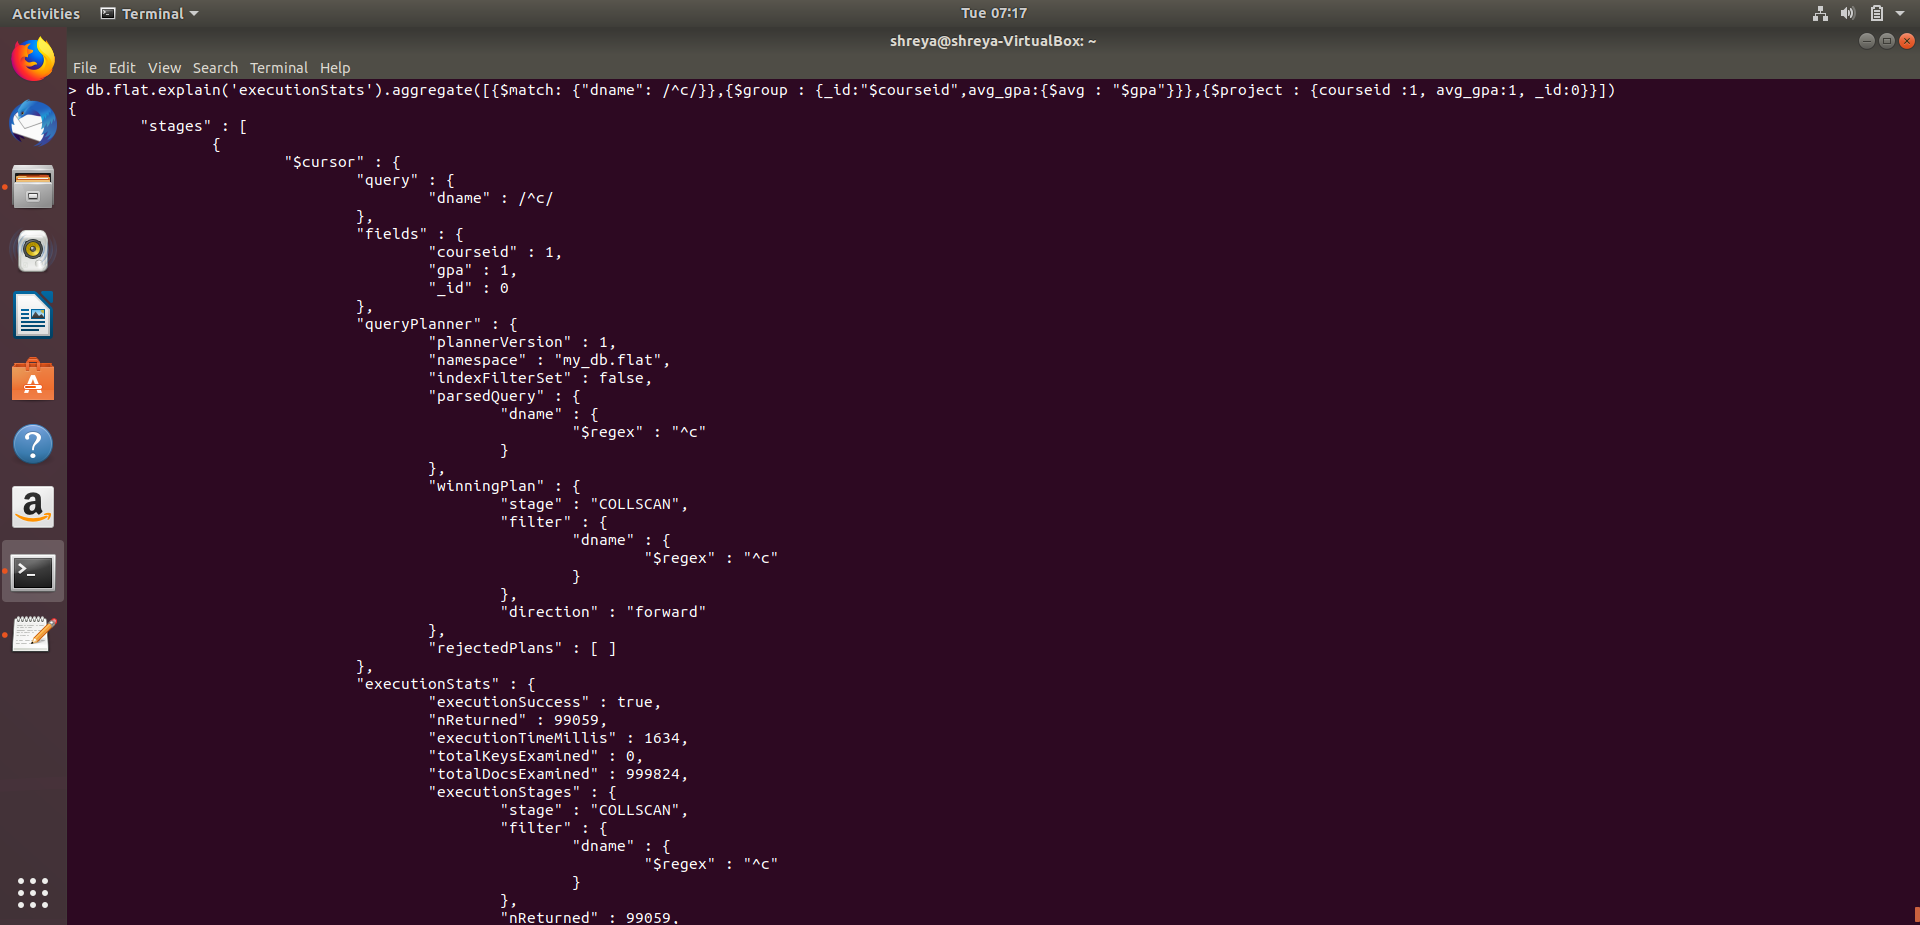
\includegraphics[scale=0.30]{mongo_2.png}

			\end{enumerate}
		\item  Improve the MongoDB query performance as below:
		\begin{itemize}
			\item Redesign the schema of the collection flat according the query Q5 such that the execution
			time of Q5 is significantly reduced. Create a new collection with your redesigned
			schema (e.g., name the new collection as nested). Transform the data from the collection
			flat to the collection nested. You can use any kind of tool or language (e.g., Java,
			Python, Apache Spark, ...) for this data transformation task. Assume in this scenario
			data redundancy is not a problem. (7 pts)
			
			
			Solution :
			We need to transform the schema such that the collection will consist of nested documents instead of flat documents. Nested documents will optimize the query and reduce the execution time significantly. The proposed optimized schema is :
			\\\{
			    \\"\_id":value
			    \\"did": value,
			    \\"dname":value,
			    \\"course":
			   \\ \{
			            \\"coursename": values,
			            \\"courseid": values
			   \\ \},
			   \\student:
			   \\ \{
			            \\"sid": values,
			            \\"gpa": values
			   \\ \}
			   
			\}
			\\The original csv file was transformed using the following code written in python which generates a json file :
			\\import pandas as pd
            \\import numpy
            $
            \\df = pd.read_csv('flat\_small.csv')
        \\def get_nested_rec(key, grp):
            \\rec = {}
            \\rec['did'] = key[0]
            \\rec['dname'] = key[1]
           \\ \#rec['coursename'] = key[2]
            \\\#nested field1=['coursename''courseid']
            \\rec['course']={}
            \\dict1={}
            \\for field in ['coursename','courseid']:
                \\dict1=list(numpy.array(grp[field].unique()))
                \\rec['course'][field]=dict1
                \\dict1={}
            \\\#nested key-val pair
            \\rec['student'] = {}
            \\dict1={}
            \\for field in ['sid','gpa']:
                \\dict1=list(numpy.array(grp[field].unique()))
                \\rec['student'][field]=dict1
                \\dict1={}
                \\return rec
                    \\records = []
            \\for key, grp in df.groupby(['did','dname']):
               \\ rec = get_nested_rec(key, grp)
                \\records.append(rec)
            \\records = dict(data=records)
            \\records
            \\with open('result_opt.json', 'w') as fp:
                    \\json.dump(str(records),fp,indent=4,ensure_ascii=False)
            $
            
			\item Write a new MongoDB query Q6 on the new collection nested which satisfies the same
			requirement in 5.2.1(b) as Q5. Provide the query execution time of Q6. (2 pts)
				$
				\\db.flat.explain('executionStats').aggregate([
				\\\{\$match: 
				    \\\{"dname":
				    /\string^c/\}\},\{\$unwind : "\$student.gpa"\},\{\$group : \\\{\_id:"\$course.courseid",avg\_gpa:
				    \\\{\$avg : "\$student.gpa"\}\}\},
				    \\\{\$project : \{\_id:1, avg\_gpa:1, \}
				\\\}])
				$
				The query execution time is less than a millisecond as it fetches only one document from the collection.

		\end{itemize}
       \item  (Continue with first task 5.2.1). Build index(es) on the collection flat to improve the performance
       of Q5. Provide the new query execution time of Q5. Note MongoDB will automatically
       create an index on id. (2 pts)
       
       Solution:
       Creating an index on did, dname and \_id (which is by default) will reduce the execution time of the query.
       \\step 1:
       \\create ascending indexes on collection:
       \\db.createIndex(\{did:1,dname:1,\_id:1\})
       \\ Compute execution time:
       The execution time was computed to be 1402 seconds, which is less than 1654 needed for non index execution.
       
       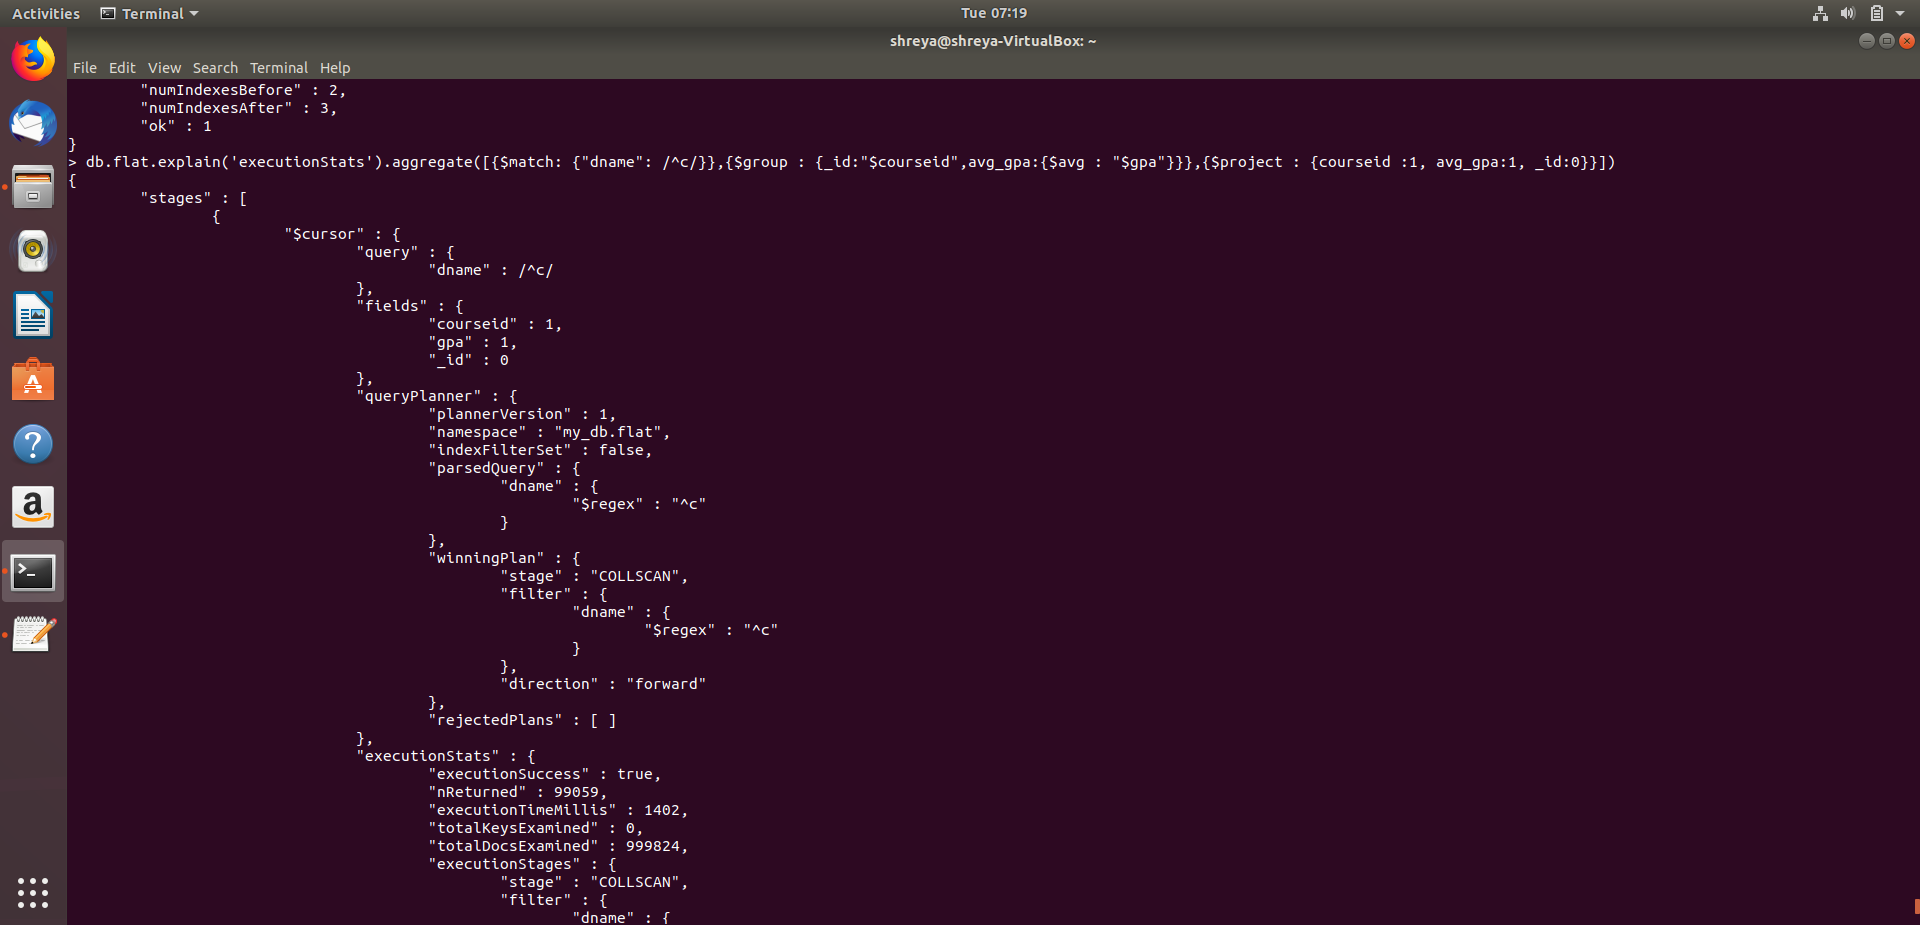
\includegraphics[scale=0.30]{mongo_4.png}
       
       
		\end{enumerate}
		
		
	
		\clearpage
	\subsection*{Exercise 5.3 (Short Questions)}
	Answer the following questions:

	\begin{enumerate}
		\item Explain the concept of ”Polyglot Persistence” in NoSQL systems? (2 pt.)\\
	Polyglot persistence facilitates use of most suitable database technology based on the requirement of an application. Different kinds of data are best dealt with different data stores. There are numerous databases available to solve different problems. Using a single database to satisfy all of a program's requirements can result in a non-performant solution.\\
	 Example:  Relational database are good at enforcing relationships that exist between various data tables. To discover a relationship or to find data from different tables that belong to the same object, an SQL join operation can be used. This might work when the data is smaller in size but becomes problematic when the data involved grows larger. A graph database might solve the problem of relationships in case of Big Data, but it might not solve the problem of database transactions, which are provided by RDBM systems. Instead, a NoSQL document database might be used to store unstructured data for that particular part of the problem. Thus different problems are solved by different database systems, all within the same application.
		
		
		\item Consider a document-oriented database with documents in the following form: (3 pt.)\\
		{ type: “invoice”, invoiceid: 5748, total : 25.0, billingcountry : “Germany” }\\
		{ type : “invoiceline”, lineid : 4378, invoiceid : 12234, trackid : 23, price : 0.99, quantity: 1
		}
\\
	{ type : “track”, trackid : 1234, name : “Let There Be Rock”, albumid : 45 }\\
	Provide the corresponding Map and Reduce functions for the following query:\\
	\textbf{Compute the average invoice total of all invoices from Germany.}\\
	\textbf{Note}: The input to the map function is one document collection which contains all objects
	of the database, regardless of their type. Hint: it is also possible, to create multiple map /
	reduce functions, where the output of the previous reduce task is the input of the next map
	task.Provide a sketch for the MapReduce implementation of these queries using some form
	of Java/JavaScript pseudo code, similar to the syntax used in the lecture.
		
	\begin{lstlisting}
	map=function() 
	{ 
		if(this.invcs!=null && this.invcs.billingcountry=="Germany")
		{
			this.invcs.forEach(function(item) 
			{ 
				emit(i.invoiceid, { sum: total.qty }); 
			}
		}
	}
	
	
	reduce=function(key, values) 
		{
			var s=0, count=0;
			values.forEach(function(value) { s+=value.sum; count++;});
			return ( { sum: s}/count );
		}
	
	\end{lstlisting}
			
		
		
	\end{enumerate}
	
  
\end{document} 
